\begin{figure}[h!]
\begin{center}
    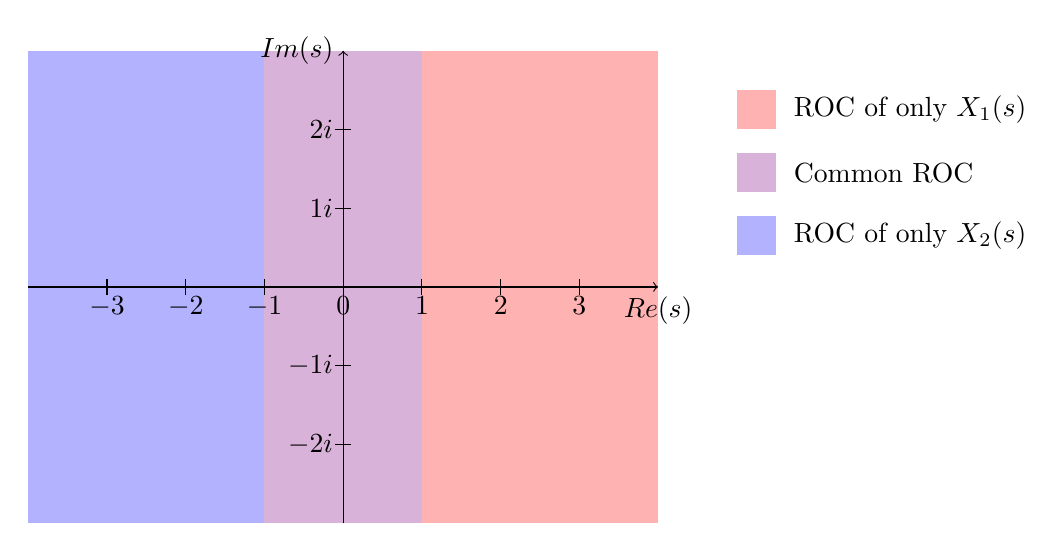
\begin{tikzpicture}
    \fill[red!30] (1,-3) rectangle (4,3);
    \fill[violet!30] (-1,-3) rectangle (1,3);
    \fill[blue!30] (-4,-3) rectangle (-1,3);
    % Axis length
    \draw[->] (-4,0) -- (4,0) node[below] {$\text{Re}(s)$};
    \draw[->] (0,-3) -- (0,3) node[left] {$\text{Im}(s)$};
    % X-axis
    \foreach \x in {-3,-2,-1,0,1,2,3}
        \draw (\x,-0.1) -- (\x,0.1) node[below=3pt] {$\x$};
    % Y-axis
    \foreach \y in {-2,-1,1,2}
        \draw (-0.1,\y) -- (0.1,\y) node[left=3pt] {$\y i$};
    % Legend
    \begin{scope}[shift={(5,2)}]
        \fill[red!30] (0,0) rectangle ++(0.5,0.5);
        \node[right] at (0.6,0.25) {ROC of only $X_1(s)$};
        \fill[violet!30] (0,-0.8) rectangle ++(0.5,0.5);
        \node[right] at (0.6,-0.55) {Common ROC};
        \fill[blue!30] (0,-1.6) rectangle ++(0.5,0.5);
        \node[right] at (0.6,-1.35) {ROC of only $X_2(s)$};
    \end{scope}
\end{tikzpicture}
\caption{Representation of ROCs of $X_1(s)$ and $X_2(s)$} \label{fig:ee23-b1}
\end{center}
\end{figure}
